\documentclass{article}
\usepackage[utf8]{inputenc}

\usepackage{graphicx}
\graphicspath{ {resources/} }

\usepackage{minted}
 
\usepackage{verse}

\usepackage{epigraph}
\setlength{\epigraphwidth}{0.25\textwidth}

\title{Lesson}
\author{Rushi Shah}
\date{May 2016}

\begin{document}

\maketitle

\epigraph{I look like a thumb.}{Kathryn Wen}

\section{Formatting}

Lists: 

\begin{itemize}
  \item \textit{Italics}
  \item \textbf{Bolding}
\end{itemize}

\section{Poetry??}
\begin{verse}
The yellow banana \\
\vin Peel \ldots \\!

The green apple \\
\vin Munch! \\!

The aggressive pineapple \\
\vin \textbf{Ouch}; \\!

Spongebob, squarepants.

\end{verse}

\section{Images}

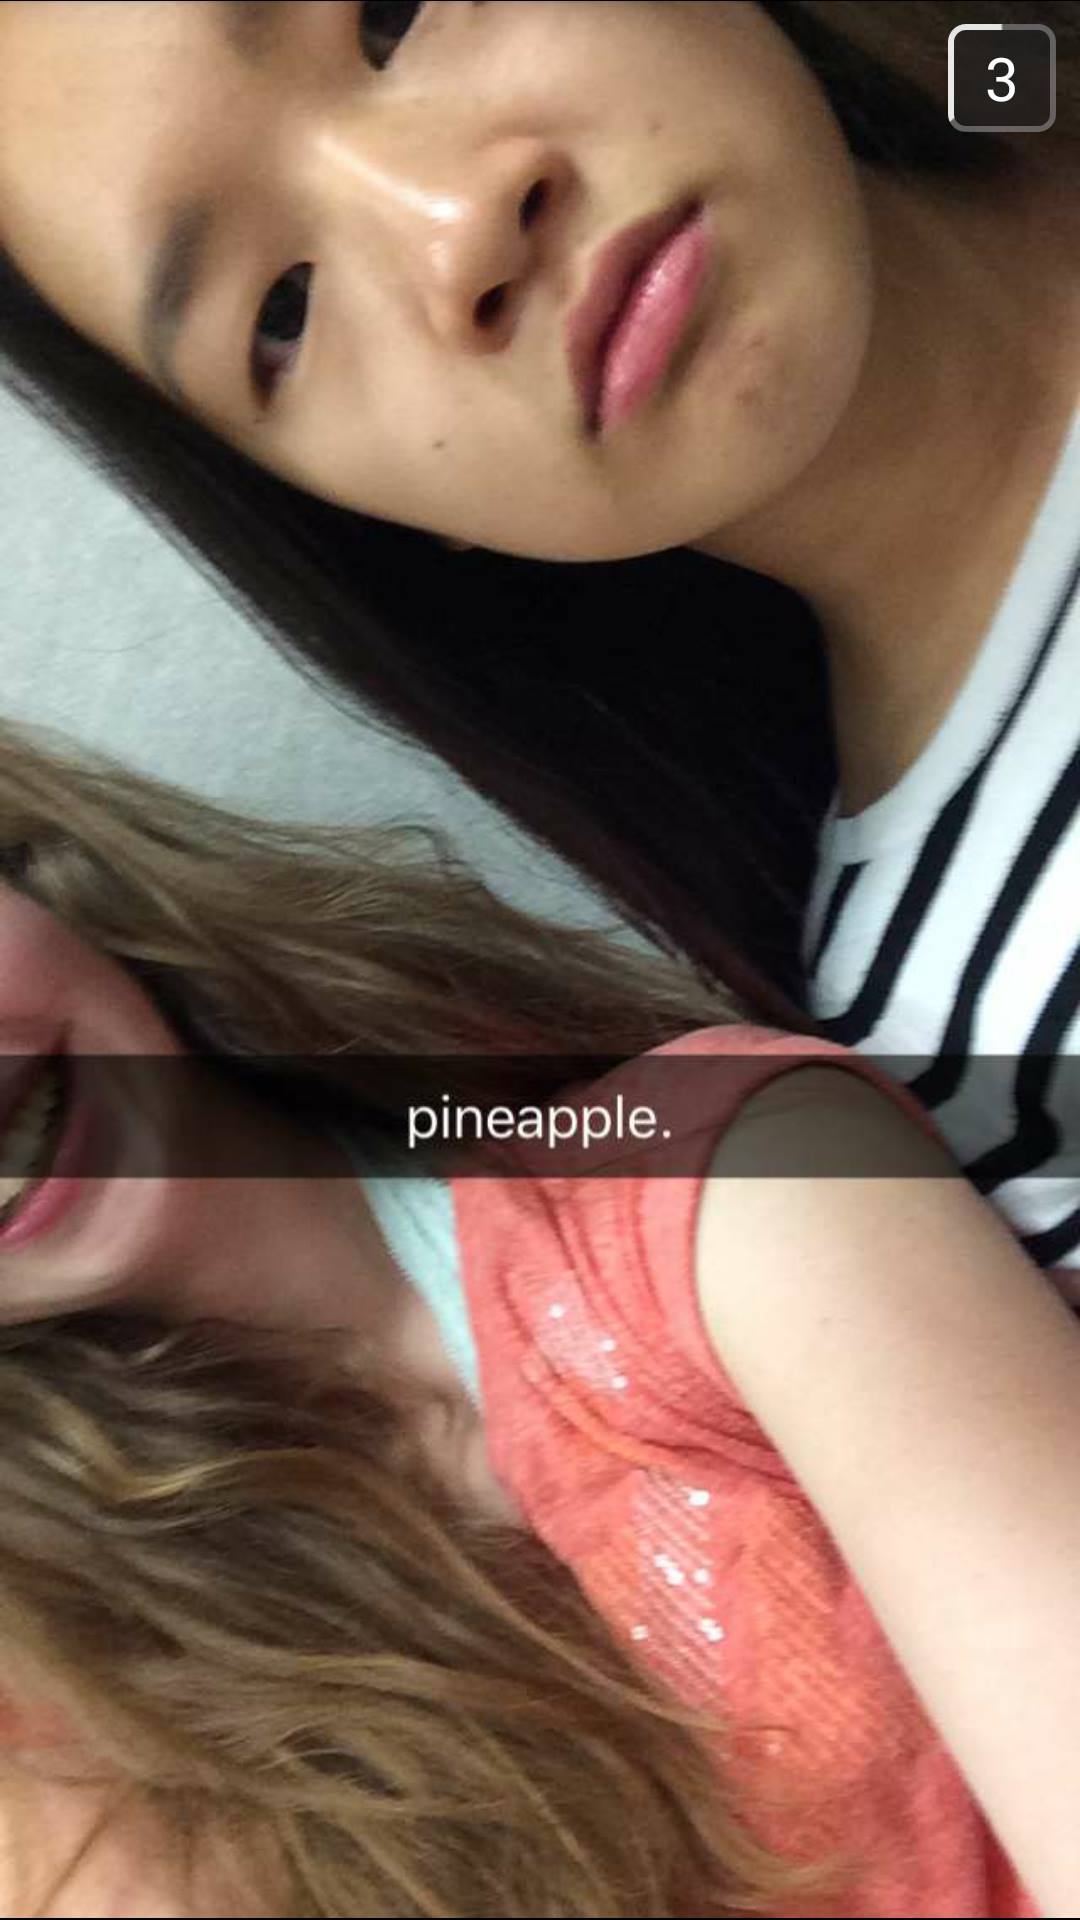
\includegraphics[height=3in]{pineapple}

\section{Math}

Math is hard. The Pythagorean theorem inline is \(x^2 + y^2 = z^2\). If you want to make a bigger deal about it, you can also do:

\[a^2 + b^2 = c^2\]

\section{Code}

Syntax highlighting looks fancy. This is a bit of code we wrote earlier this year:

\begin{minted}{javascript}
app.get('/greet/:name', function(req, res){
  res.send("Hello there, " + req.params.name + ".");
});

var server = app.listen(process.env.PORT, function () {
  var host = server.address().address;
  var port = server.address().port;

  console.log('Example app listening at http://%s:%s', host, port);
});
\end{minted}

\end{document}
